\begin{nestedsection}{CoDeR Model for Continuous Deductive Reasoning}{model}
	CoDeR is an abstract model for continuous deductive reasoning over streamed RDF data that expresses the semantics of Continuous Datalog, thus supporting continuous reasoning expressed in both RIF-Core and OWL 2 RL.
	It is composed of a stream-based data model for expressing the streams $S$, $P$ and $N$ of each ${\Pi^{C,r} = \langle R,F^0,S,r \rangle \models \langle E^0,P,N \rangle}$, and a minimal algebra of stream-to-stream operators for expressing the persistent set of rules $R$.
	It casts the problem of applying those rules to streamed RDF data as that of iterative pattern matching, in a manner inspired by the Rete pattern matching algorithm \citep{forgy79}, though it is meant to support any such algorithm rather than prescribing one itself.

	% Stream-based Data Model
	\begin{nestedsection}{Data Model}{model: data}
		The data model of CoDeR is composed of multiple-source multiple-sink streams.
		These streams are divided into two classes: \emph{input}/\emph{output} streams and \emph{inter-operator} streams.

		In the first case, input/output streams provide the semantics of the streams $S$, $P$ and $N$ for any $\Pi^{C,r}$ expressed by a CoDeR-based system.
		These streams are sequences of instances of heterogeneous RDF graphs compatible with the ongoing work on query semantics by the RSP working group\footnote{\url{https://github.com/streamreasoning/RSP-QL/blob/master/Semantics.md}};
		an instance of an RDF graph is an RDF graph annotated with a time interval ${(e,n]}$: ${\langle \{(s,p,o),\dots,(s',p',o')\},e,n \rangle}$.
		As the atomic units of Continuous Datalog are instances of facts, being triples in RDF, graph instances arriving on the input stream must be translated into sequences of fact instances using the graph-to-triples operator described in \refsec{model: algebra}, where each fact instance inherits the time interval of the graph instance in which it originated.

		The interval ${(e,n]}$ for any graph or triple instance is the the period of time for which the data is \emph{valid} \citep{SemanticStreamingManagement,sparkwave} according to the ${\Pi^{C,r} = \langle R, F^0, S, r \rangle}$ expressed.
		For graphs on the input stream, $e$ is the instant at which a given graph was asserted, and ${n = e + r}$ is the instant at which it will leave the semantic sliding window over $S$ of $\Pi^{C,r}$ (or become ``negated'').
		For graphs on the output stream, $e$ is the latest instant at which any part of the justification of a given graph was asserted, and $n$ is the earliest instant at which any part of its justification will leave the sliding window.
		\reffig{intersected-intervals} provides an example of this for some ${\Pi^{C,r} = \langle \{c \Leftarrow a \land b\},\{\},[\langle a,1 \rangle,\langle b,2 \rangle ], 3\rangle}$ over instants ${i = 1 \dots 4}$.
		\begin{figure}
			\centering
			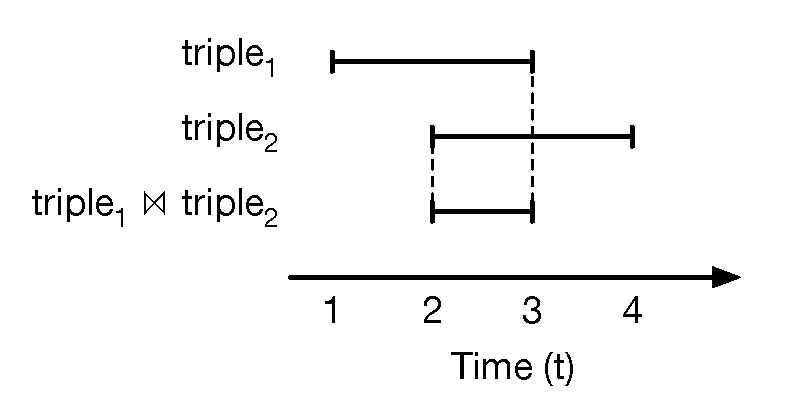
\includegraphics[width=0.3\textwidth]{intersected-intervals}
			\caption{Derivation of valid-time for entailed fact instance from those of its justification.}
			\labelfig{intersected-intervals}
		\end{figure}
		\begin{align*}
			\Pi^{C,r}_{1} & = \langle \{c \Leftarrow a \land b\}, \{ \langle a, 1 \rangle \} \rangle & \models & \{ \} \\
			\Pi^{C,r}_{2} & = \langle \{c \Leftarrow a \land b\}, \{ \langle a, 1 \rangle, \langle b, 2 \rangle \} \rangle & \models & \{ \langle c, 2 \rangle \} \\
			\Pi^{C,r}_{3} & = \langle \{c \Leftarrow a \land b\}, \{ \langle a, 1 \rangle, \langle b, 2 \rangle \} \rangle & \models & \{ \langle c, 2 \rangle \} \\
			\Pi^{C,r}_{4} & = \langle \{c \Leftarrow a \land b\}, \{ \langle b, 2 \rangle \} & \models & \{ \}
		\end{align*}
		It is clear that a CoDeR output stream expresses the semantic stream $P$ entailed by some $\Pi^{C,r}$.
		However, as the semantic stream $N$ is defined as the sequence of entailments of some $\Pi^{C,r}$ ordered by the instant $n$ at which $W^{S,r}_{n}$ \emph{ceased} to justify them, the output stream of a CoDeR-based system also expresses the stream $N$.
		As such, the annotation of streamed RDF graphs with the interval $(e,n]$ gives the streams of CoDeR a dual semantics with regard to Continuous Datalog.

		In the second case, inter-operator streams are produced and consumed by the stream-to-stream operators of CoDeR's minimal algebra.
		These streams are sequences of the intermediate results of processing between steps in the production of entailments.
		As the production of entailments in CoDeR is cast as an iterative pattern matching problem, all intermediate results of this process will also take the form of instances of RDF graphs;
		an inter-operator stream is a sequence of instances of homogeneous RDF graphs, each matching the same graph pattern, that being a sub-pattern of the body of one of the rules $R$ of the expressed $\Pi^{C,r}$.
		These instances of RDF graphs could be considered to be ``entailed'' by the sub-pattern of the stream on which they appear and the presence of valid instances of their constituent RDF triples within the system;
		as such, the same dual semantics of valid-times may be applied to these intermediate matches as to the true entailments of the model found on output streams.
		It follows that inter-operator streams are functionally the same as input/output streams, only being distinct in their semantics:
		the former are sequences of homogeneous RDF graphs that hold no value outside of a system, while the latter contain heterogeneous graphs that are either the entailments of the system or the assertions of its predecessor in the stream pipeline.

		In addition, each stream in the model is semantically distinct:
		each input/output stream is from a distinct source and uniquely identifiable by the source's IRI;
		each inter-operator stream contains graphs matching a specific graph pattern and are uniquely identifiable by that pattern.
		As the same graph pattern may be a sub-pattern of many rule bodies, and so appear in multiple places in a processing plan, one inter-operator stream may be the input to multiple operators.
		Furthermore, two or more operators may contribute to the same stream within the model, where the pattern of the stream in question is the union of the patterns of the streams produced by each of the operators in isolation.
		In this case, each operator contributes results to the common stream as they are produced, passively interleaving the streams produced by the individual operators such that the resultant stream is still ordered by the entailment instant $e$ of the constituent instances.
		As this is the active behaviour of a stream union operator, such an operator is not needed in CoDeR.
		However, within the algebra of CoDeR, such a stream is still denoted ${op_{application} \cup op_{application}}$.
	\end{nestedsection}

	% Minimal Algebra
	\begin{nestedsection}{Minimal Algebra}{model: algebra}
		The minimal algebra of CoDeR is based on that of Positive Datalog, that being ${\{\bot, \text{:-}, \wedge\}}$.
		Of these, implication $\text{:-}$ and conjunction $\wedge$ may be expressed as stream-to-stream operators, the former being extended to apply to instances as $\text{:-}_{head}$ and the latter being the window-join $\Join$ \citep{niagaraCQ}, in order to support forward-chaining processing of fixed rules;
		$\bot$ is not an operator, but the special class of values that should not exist, represented in CoDeR by the ${rif\text{:}error()}$ class from RIF \citep{w3crif}.
		% Further, in order to support both fixed-plan pattern-matching algorithms such as the Rete algorithm \citep{forgy79} and adaptive algorithms such as the Eddies algorithm \citep{eddies} and its derivatives \citep{CACQ,TCQ}, CoDeR replaces the window-join operator with the State Module of Eddies, algebraically represented by ${{}_b\Join_p}$.
		Further, in order to support both fixed-plan pattern-matching algorithms such as the Rete algorithm \citep{forgy79} and adaptive algorithms such as the Eddies algorithm \citep{eddies} and its derivatives \citep{CACQ,TCQ}, CoDeR replaces the window-join operator with the State Module of Eddies, which we represent algebraically by $\rstreamjoin$.
		% In addition to $\text{:-}_{head}$ and ${{}_b\Join_p}$, CoDeR utilises a pair of stream-filter operators, $\sigma_{triple}$ and $\sigma_{external}$, for identifying \emph{basic patterns} as defined in SPARQL \citep{w3csparql} and expressing the datatype functions of RIF-Core \citep{w3crifcore}, respectively.
		In addition to $\text{:-}_{head}$ and $\rstreamjoin$, CoDeR utilises a pair of stream-filter operators, $\sigma_{triple}$ and $\sigma_{external}$, for identifying \emph{basic patterns} as defined in SPARQL \citep{w3csparql} and expressing the datatype functions of RIF-Core \citep{w3crifcore}, respectively.
		Finally, as basic patterns match individual triples and CoDeR's streams are composed of graphs, the CoDeR algebra includes a graph-to-triples operator ${{}_g\pi_t}$ to translate input streams to the streams of triples on which $\sigma_{triple}$ operates.
		% In summary, the minimal algebra of CoDeR consists of the set of operators ${\{\text{:-}_{head}, {}_b{\Join_p}, \sigma_{triple}, \sigma_{external}, {}_g{\pi_t}\}}$.
		In summary, the minimal algebra of CoDeR consists of the set of operators ${\{\text{:-}_{head}, \rstreamjoin, \sigma_{triple}, \sigma_{external}, {}_g{\pi_t}\}}$.

		As all operators are stream-to-stream in nature, they each take one or two streams as input and produce a single stream (though they may contribute to any number of union streams).
		As such, the notation for applying an operator to a stream is also the definition of a stream, and may, therefore, be used as input to another operator.
		For example, \refeqn{basic-example-plan} is a plan expressed in the CoDeR algebra for the ${\Pi^{C,r} = \langle \{b \Leftarrow a\}, \{\}, S, r \rangle}$, where $a$ and $b$ are RDF triples.
		\begin{equation}\labeleqn{basic-example-plan}
			\text{:-}_b \left( \sigma_a \left( {}_g{\pi_t}\,S \right) \right)
		\end{equation}

		\begin{description}
			\item[$\sigma_{triple}\,X$] \hfill \\
				\begin{figure}[t]
					\centering
					
\includegraphics[width=0.3\textwidth]{basic-pattern-match}
					\caption{The triple-select operator.}
					\labelfig{continuous datalog: basic pattern match}
				\end{figure}
				The triple-select operator identifies instances of triples in a stream $X$ that match some \emph{basic pattern} \citep{w3csparql}.
				This operator is semantically equivalent to the \emph{basic pattern match} of SPARQL applied to a stream, and to the \emph{alpha nodes} of the Rete pattern matching algorithm \citep{forgy79} applied to semantic data.
				Like these operators, the triple-select is one-pass, and so is trivially interpreted as the unary stream-to-stream operator $\sigma_{triple}$, where ${triple}$ is the basic pattern to be matched.
				It takes an inter-operator stream $X$ of triple instances as input and produces an inter-operator stream of triple instances, where the produced stream contains a subset of those instances in the input stream, maintaining the ordering of those instances.
				The contents of the produced stream are characterised as those triple instances from the input stream whose triples match the specified basic pattern.
			\item[$\sigma_{external}\,X$] \hfill \\
				\begin{figure}[b]
					\centering
					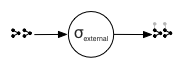
\includegraphics[width=0.3\textwidth]{datatype-function}
					\caption{The operator encompassing all datatype functions of RIF-Core.}
					\labelfig{continuous datalog: datatype function}
				\end{figure}
				This operator encompasses all of the one-pass built-in datatype functions of RIF-Core, and is also trivially interpreted as a unary stream-to-stream operator $\sigma_{external}$, where ${external = f(a_1,\dots,a_n)}$, $f$ is the datatype function to apply and each $a_i$, ${1 \leq i \leq n}$ is either a variable or a constant value to which $f$ is to be applied.
				It filters elements of its input stream $X$ based not on the semantic structure of the data but directly on the values of variables, which are consistent throughout any given graph pattern;
				thus the $\sigma_{external}$ operator expresses an \emph{advanced} component of an \emph{advanced graph pattern}, as specified in SPARQL.
				As such, it takes an inter-operator stream $X$ of graph instances as input and produces an inter-operator stream of graph instances, where the produced stream contains a subset of those instances in the input stream, maintaining the ordering of those instances.
				The contents of the produced stream are characterised as those graph instances from the input stream whose graphs match a specific advanced graph pattern.
			\item[${{}_g{\pi_t}\,X}$] \hfill \\
				\begin{figure}[t]
					\centering
					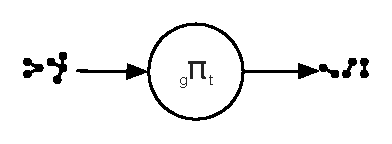
\includegraphics[width=0.3\textwidth]{graph-to-triple}
					\caption{The graph-to-triple operator.}
					\labelfig{continuous datalog: graph-to-triple}
				\end{figure}
				The graph-to-triples operator ${{}_g{\pi_t}}$ is a unary operator that deconstructs graph instances into sequences of triple instances, the union of the triples instantiated therein being equal to the contents of the original graph.
				It takes a heterogeneous (\emph{input/output}) stream $X$ of RDF graph instances and produces a homogeneous (\emph{inter-operator}) stream of RDF triple instances.
				Each triple instance produced is assigned the same valid-time interval as the graph instance in whose graph the instantiated triple was contained.
				Consider, for example, the input/output stream containing an instance of a graph containing the RDF triples $a$ and $b$ and valid from instant $t_e$ to instant $t_n$:
				\begin{multline*}
					{}_g{\pi_t} (\dots,\langle \{a,b\},t_e,t_n \rangle,\dots) = \\
						(\dots,\langle a,t_e,t_n \rangle,\langle b,t_e,t_n \rangle,\dots)
				\end{multline*}
			\item[$\text{:-}_{head}\,X$] \hfill \\
				\begin{figure}[b]
					\centering
					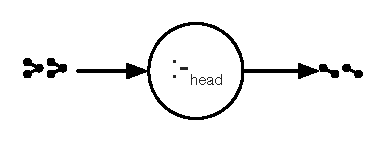
\includegraphics[width=0.3\textwidth]{instance-implication}
					\caption{The instance implication operator.}
					\labelfig{continuous datalog: instance implication}
				\end{figure}
				Instance implication is a one-pass operator that takes as input an inter-operator stream $X$ whose graph pattern is the body of one of the rules $R$ of the expressed $\Pi^{C,r}$, and produces an inter-operator stream whose graph pattern is the head of that axiomatic rule.
				Each graph instance received on the input stream causes the production of a single graph instance that matches the pattern of the head clause and is populated with the bindings of the received instance.
				This is similar to the CONSTRUCT clause of SPARQL, or the final step of \emph{conflict set resolution} within the Rete algorithm \citep{forgy79}.
				In addition, each produced instance inherits its valid-time interval from the graph instance that implied it.
			% \item[${S_1\,{}_b{\Join_p}\,S_2}$] \hfill \\
			\item[${X\,\rstreamjoin\,Y}$] \hfill \\
				\begin{figure}[t]
					\centering
					\subfloat[The SteM operator.]{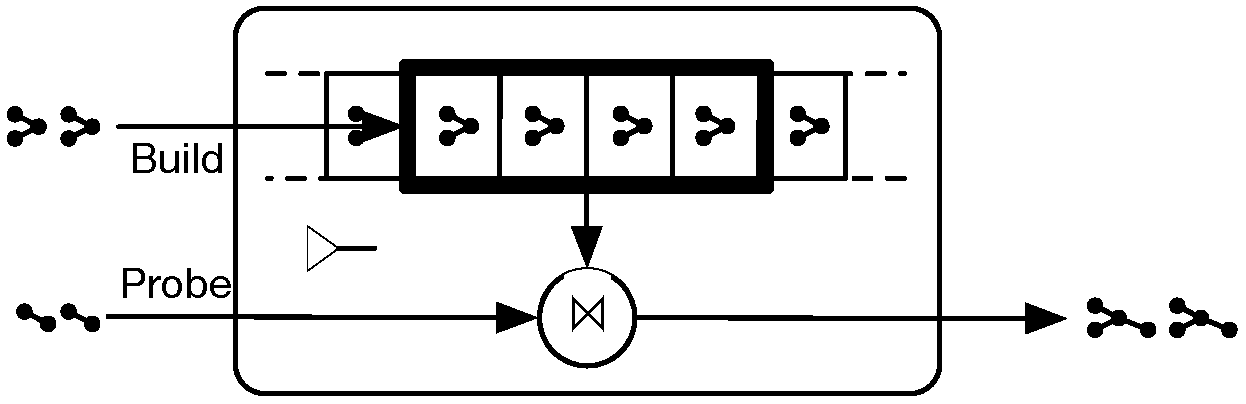
\includegraphics[width=0.45\textwidth]{SteM}}\\
					\subfloat[A typical window-join.]{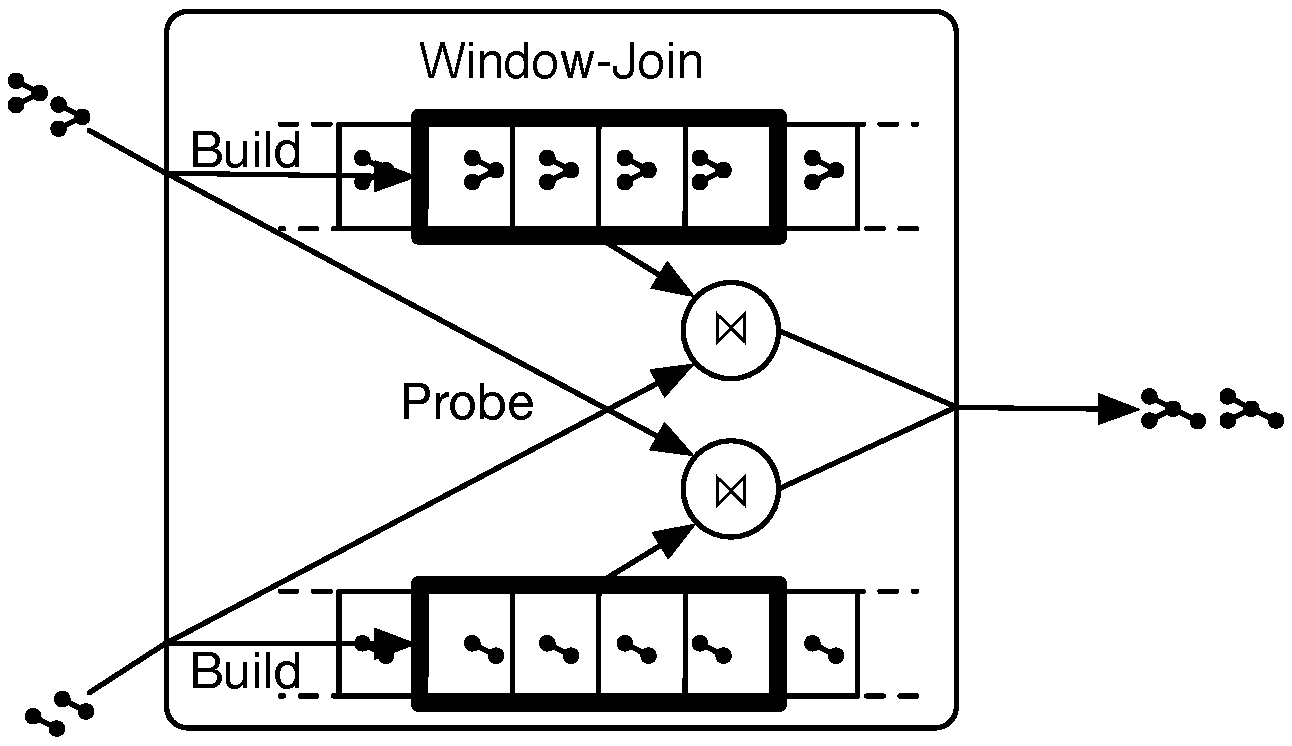
\includegraphics[width=0.45\textwidth]{window-join}}
					\caption{Exploded views of two-pass joining operators.}
					\labelfig{continuous datalog: SteM}
				\end{figure}
				State Modules (\emph{SteM}s) are asymmetrical binary operators that each perform the dual function of maintaining a window of graph instances and ``joining'' each graph instance on a stream against those within the maintained window (known as ``probing'' the window).
				These are the same two functions performed for each window in a symmetric window-join, extended from Rete \emph{beta nodes} in \citep{ReteDBMS}, with results of each probe being produced to the same result stream as they occur.
				Window-joins are, therefore, functionally identical to the union of two complementary SteMs:
				% ${A \Join B = \left( A\,{}_b{\Join_p}\,B \right) \cup \left( B\,{}_b{\Join_p}\,A \right)}$, where $A$ and $B$ are inter-operator streams.
				${A \Join B = \left( A\,\rstreamjoin\,B \right) \cup \left( B\,\rstreamjoin\,A \right)}$, where $A$ and $B$ are inter-operator streams.
				In addition, it should be noted that SteMs express the semantics of the sequential intersection operator ${seq}$ proposed in EP-SPARQL \citep{EP-SPARQL}, in that they join new data from one stream with the prior (valid) contents of another, thereby supporting rudimentary event processing.

				The implementations of SteMs in the literature show a great variety of behaviour regarding window maintenance \citep{SteMs}, in the most extreme case ceasing to be a wholly stream-to-stream operator and supporting the incorporation of ``static'' data into stream processing systems.
				In the minimal algebra of CoDeR, however, SteMs simply support the building of a \emph{valid window} (as defined in \refsec{semantics}) from its first inter-operator stream $X$, and the probing of that window with data from its second inter-operator stream $Y$ to produce an inter-operator stream of the homogeneously joined graph instances.
				Furthermore, the nature of probing in CoDeR is strictly limited to that of the natural join between the variables in the patterns for streams $X$ and $Y$.
				Finally, in contrast to the direct inheritance of valid-times in unary operators of CoDeR, the valid-time interval assigned to each graph produced by a SteM is the intersection of the valid-times of the two joined graphs.
		\end{description}

		% As the SteM ${{}_b{\Join_p}}$ is the only CoDeR operator that maintains any form of window over its input, and SteMs maintain exclusively \emph{valid windows}, no data will persist within a CoDeR-based system when it is no longer valid according to its annotations.
		As the SteM $\rstreamjoin$ is the only CoDeR operator that maintains any form of window over its input, and SteMs maintain exclusively \emph{valid windows}, no data will persist within a CoDeR-based system when it is no longer valid according to its annotations.
		Furthermore, the valid-time interval of any instance is either directly inherited from the interval of the input instance, in the case of one-pass operators, or derived from the intersections of the intervals of both contributing instances in the sole two-pass operator, the SteM;
		as such, it is guaranteed that all instance annotations accurately describe the intervals for which the given instance is justified by the contents of the semantic sliding window of range $r$ over the system input streams $S$ defined in a given ${\Pi^{C,r} = \langle R,F^0,S,r\rangle}$.
		It follows that no facts may persist in a CoDeR based system if it is no longer valid, and thus only entailments that are valid at a given moment may be produced in that moment, thereby guaranteeing correct results according to the semantics of Continuous Datalog.
		It also follows that, given a system with a processing plan that is expressible in the CoDeR algebra and accurately represents a set of rules $R$ of a $\Pi^C$, all fact instances that are logically entailed by that $\Pi^{C,r}$ at a given instant will be persisted within that system at that instant,
		i.e. such a CoDeR-based system is guaranteed to produce the complete set of results according to the semantics of Continuous Datalog.
	\end{nestedsection}
\end{nestedsection}
